%!TEX root = volumeFinal.tex 
\chapter{\label{chap:planejamento}Planejamento}

A atividade de planejar alguma coisa é feita muitas vezes por dia. Algumas vezes esse planejamento é muito simples, como organizar as tarefas que serão feitas no próximo dia, outras vezes pode ser mais complexa como organizar uma viagem de final de ano. Planejar implica em elaborar uma sequência de ações com o intuito de alcançar um objetivo, ou seja, o processo de planejar consiste em organizar as ações, antecipando os resultados esperados de cada ação, com o intuito de conquistar um objetivo. 

O planejamento, na área da IA, é uma sub área de estudo, onde ele é usado para encontrar um plano que resolva um problema especifico. Como os ambientes nem sempre possuem as mesmas características, existem diferentes técnicas que são usadas para construir um plano.

\section{Planejamento automatizado}

Planejamento automatizado estuda o processo de geração de planos computacionalmente. O objetivo do planejamento é encontrar uma sequência de ações que solucione um problema, a sequência de ações encontrada é chamada de plano. Para construir um plano é utilizado um planejador. O planejador recebe uma descrição formal de um problema de planejamento, e tenta solucionar esse problema utilizando algoritmos de buscas e heurísticas \cite{ghallab2004automated, intelligence2003modern}.

\subsection{Representação de um problema de planejamento}

Uma das maneiras de representar um problema de planejamento é utilizando lógica matemática. \frm{Salto de lógica matemática para lógica proposicional.}
A lógica proposicional é expressada através de sentenças atômicas, que são compostas de proposições. 
Cada proposição pode assumir um valor de verdadeiro ou falso. 
Por exemplo, queremos representar que a lâmpada está apagada, para isso pode ser utilizado a proposição $apagada$, se a lâmpada estiver apagada, a proposição assume o valor de verdadeiro. Junto com as proposições podem ser usados conectivos lógicos, como negação (\textit{not}) $\neg$, conjunção (\textit{and}) $\wedge$ e disjunção (\textit{or}) $\vee$. 
No exemplo da luz, se queremos saber se a luz está apagada e a TV está ligada, podemos representar por $apagada~ \wedge~ ligada$. 
A lógica proposicional pode ser considerada simples, mas ela serve de base para as lógicas mais expressivas \cite{intelligence2003modern}. 

Como a lógica proposicional tem expressividade limitada, é preciso utilizar uma lógica que consiga resolver esse problema.\frm{Qual problema?} 
A lógica de primeira ordem (LPO) estende a lógica proposicional.\frm{E...?} 
Na LPO uma sentença atômica é composta por um predicado seguido de uma lista de termos, denotada por $p(t_{0}, t_{1}, ..., t_{n})$. 
Um predicado se refere a uma relação existente entre os termos. 
Os termos são objetos que se referem a objetos definidos, indefinidos ou a funções \cite{intelligence2003modern}. 
No exemplo da lâmpada, podemos dizer que a lâmpada da cozinha está apagada, representado por $apagada(cozinha)$. 
Ou ainda podemos dizer que a lâmpada do quarto está apagada e a TV da sala está ligada, $apagada(quarto)~ \wedge~ ligada(sala)$.  

\subsection{Formalização de um problema de planejamento}

Como nas técnicas de busca, em planejamento também é necessário ter uma descrição do problema.
Para realizar a descrição de um problema de planejamento é preciso definir alguns conceitos, são eles \cite{intelligence2003modern, ghallab2004automated, meneguzzi2015planning}:\frm{Evita este tipo de itemização com parágrafos no lugar de itens. Articula o texto melhor e transforma isto em um ou mais parágrafos.}

\begin{itemize}
	\item estados, onde cada estado é um predicado.\frm{Cada estado não é um predicado. Cada estado é representado por uma valoração para todos os predicados associados a todos os objetos! Lembre-se que em planning o estado é como se fosse um vetor de bits} Conforme a situação do ambiente os estados assumem os valores de verdadeiro ou falso;
	\item operadores, cada operador é definido como $op = (nome(t), pre(p), efeitos(p)$. 
	O $nome(t)$ é o nome do operador e t é o conjunto de termos que irão\frm{Tu ainda nem falou de precodições e efeitos. Igualmente, não use futuro para se referir a texto neste trabalho ou elementos que já existem. Como regra geral não use outro tempo que não o presente a não ser que tu consiga pensar muito bem nisto.} aparecer nas precondições e efeitos. $pre(p)$ é o conjunto de predicados que representam as precondições do operador. $efeitos(p)$ é o conjunto de predicados que serão o resultado após a execução do operador; e
	\item domínio, o conjunto de operadores que podem ser usados para a resolução do problema.
\end{itemize}

Os operadores também são chamados de ações.\frm{Ações e operadores, para mim, não são a mesma coisa. Uma coisa é uma instância ground, a outra é o esquema do operador (com variáveis)} 
As ações causam uma alteração no ambiente. Um exemplo é mover um objeto de um lugar para o outro, precisamos de um estado que defina que um objeto está em determinado lugar.\frm{Evitar confusão entre estado e predicado.} 
Esse exemplo é representado abaixo:

\begin{itemize}
	\item Ação(move(from, to))
	\item Precondição: at(from)
	\item Efeito: $\neg$ at(from) $\wedge$ at(to)
\end{itemize}

Uma ação $a$ é aplicável em um estado $s$, se todas as precondições forem satisfeitas no estado $s$. 
O resultado gerado pela execução de $a$ no estado $s$ é um novo estado $s'$, nesse estado é aplicado todos os efeitos, removendo os predicados negativos e adicionando os positivos.

Formalmente, um problema de planejamento pode ser descrito como $P = (\Sigma, s_{0}, g)$, onde $\Sigma$ é o domínio do problema\frm{Domínio do problema?}, $s_{0}$ é o estado inicial onde o problema começa e $g$ é o objetivo \cite{ghallab2004automated}. 
Voltando ao exemplo do Capítulo~\ref{chap:busca}, onde um agente tenta chegar a cidade de Porto Alegre partindo da cidade de São Jerônimo, podemos formaliza-lo como:

\begin{itemize}
	\item \textbf{estado inicial} ($s_{0}$) = $At(S$\~a$o~Jer$\^o$nimo)$;
	\item \textbf{objetivo} ($g$) = $At(Porto~Alegre)$; e
	\item \textbf{domínio} ($\Sigma$) = \\
	-	nome: $move(cityA, cityB)$\\
	-	precondições: $at(cityA) \wedge link(cityA, cityB)$\\
	-	efeitos: $\neg at(cityA)~ \wedge at(cityB)$.
\end{itemize}


O processo de geração do plano é feito pelo planejador. 
Um plano é uma sequência de operadores gerada a partir de um problema que, quando executada a partir do estado inicial,  modifica o estado de forma que o objetivo seja válido no estado resultante. 
A Figura \ref{fig:planmodelo} ilustra o comportamento do planejador.

\begin{figure}[ht]
	\centering
	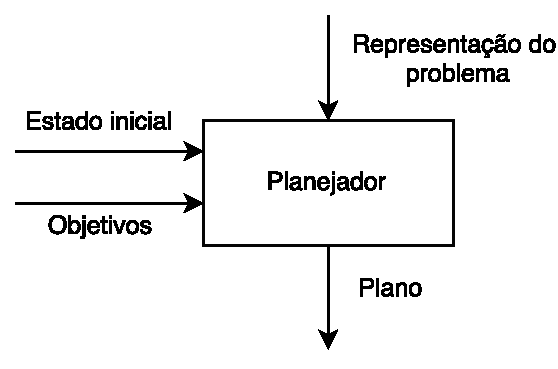
\includegraphics[width=0.4\textwidth]{fig/modelo.pdf}
	\caption{Problema de planejamento clássico.}
	\label{fig:planmodelo}
\end{figure} 

Um plano é considerado ótimo quando utiliza o menor número de ações para resolver o problema, ou seja, o número de ações que levam o estado inicial até o objetivo é o menor possível.\frm{Isto foi raciocínio circular. Talvez tu queira dizer que não há nenhum outro plano que atinga o objetivo utilizando um número menor de ações} 
Para gerar planos ótimos o planejador utiliza técnicas de busca combinado com alguma heurística que seja independente de domínio.\frm{Nem sempre existem heurísticas envolvidas (e.g. SAT), dá uma revisada nos meus slides de planejamento, ou pede os meus slides de planejamento automático.} 
Uma heurística deve ser computacionalmente eficiente e ter precisão para que a geração do plano seja eficiente \cite{helmert2007flexible}. %\frm[color=yellow]{E...? Terminar a seção numa figura, sem conectar com o resto do trabalho?}

\section{Planejamento hierárquico} 


Embora que o planejamento clássico consiga gerar planos ótimos, a quantidade de ações resultante\frm{A quantidade de ações resultantes?!?! Como assim? Tu queres dizer que problemas de grande complexidade ou com espaços de estado/busca grandes podem ser intratáveis.} é grande para problemas maiores. 
O planejamento clássico possui uma expressividade limitada, pois não é possível representar quando uma ação irá ocorrer, por exemplo~\cite{intelligence2003modern}.\frm{Coloca o til entre o texto e a citação para ser um non-breakable space.} 
Como alternativa para esses problemas foi proposto o planejamento hierárquico, chamado de \textit{Hierarchical Task Network} (HTN). 
O planejamento HTN se diferencia do planejamento clássico na forma como os planos são gerados~\cite{ghallab2004automated}. 
Enquanto no planejamento clássico é necessário ter heurísticas para a geração de planos, em planejamento HTN é possível expressar conhecimento de domínio junto com os operadores, isso faz com que as ações sejam tratadas em mais alto nível \cite{intelligence2003modern}.  

\frm[inline]{Se possível, fale um pouco mais sobre conhecimento de domínio}

O objetivo do planejamento HTN é produzir uma sequência de ações que executam determinada tarefa $t$. 
As tarefas são completadas decompondo tarefas não primitivas em tarefas menores até só restarem tarefas primitivas.  
As tarefas primitivas são análogas as ações executáveis em planejamento clássico, e expressam uma atividade que o agente possa executar diretamente no ambiente~\cite{intelligence2003modern}. 
Já as tarefa não primitiva representam objetivos que o agente deve alcançar com o intuito de decompor as tarefas não primitivas em primitivas. 
O exemplo da seção anterior de mover um objeto de lugar é um exemplo de tarefa primitiva, pois altera o estado do ambiente, podendo ser representado em HTN como: $(move~ ?from~ ?to)$. 
Um exemplo de tarefa não primitiva é realizar uma viagem de carro, para conseguir completar essa tarefa é necessário fazer a revisão do carro, arrumar as malas e colocar tudo dentro do carro, que pode ser representado por $(travelByCar ~?car~ ?stuffs))$. 

Para iniciar a geração de um plano HTN, deve ser usado como início uma tarefa de ligação. 
Uma tarefa de ligação HTN é definida como $w = (T, C)$, onde $T$ é um conjunto de tarefas a ser completadas e $C$ é um conjunto ordenado de restrições sobre as tarefas $T$. 
As restrições estabelecem a ordem com que as tarefas $T$ devem ser executadas. 

Um domínio de planejamento HTN é um par $D = (A, M)$, onde $A$ é um conjunto de predicados, que representam estados no ambiente, e $M$ um conjunto finto de métodos \cite{meneguzzi2015planning}. 
Um método é utilizado para decompor tarefas não-primitivas em primitivas. 
Um método é representado por $m = (p, t, w)$, onde $p$ é uma precondição que estabelece o que deve estar presente no estado atual para que a tarefa $t$ consiga ser decomposta por uma tarefa de ligação $w$ \cite{ghallab2004automated}. 
Considerando o exemplo anterior de viajar de carro, a Figura~\ref{fig:htnmethod} ilustra esse método, sendo a tarefa em cinza uma tarefa não primitiva, que posteriormente também será decomposta. 
O conjunto de tarefas que faz parte da tarefa de ligação está representada pelas sub tarefas, e a ordem caracteriza as restrições. 

\begin{figure}[ht]
	\centering
	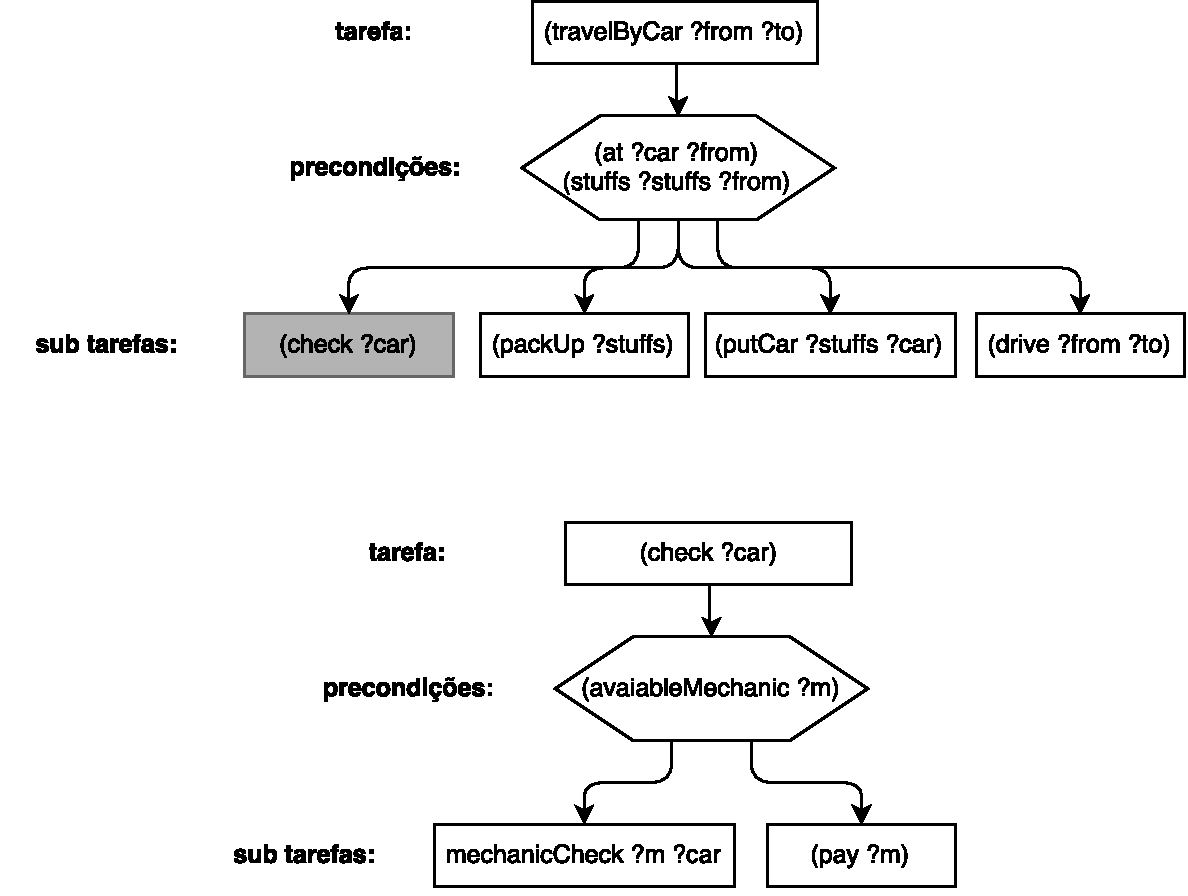
\includegraphics[width=0.7\textwidth]{fig/htnmethod.pdf}
	\caption{Exemplo de método HTN.}
	\label{fig:htnmethod}
\end{figure} 

Um problema de planejamento HTN $P$ é definido como $P = (d, I, D)$, onde $D$ é um domínio, $d$ é a tarefa de ligação inicial e $I$ é um estado inicial como no planejamento clássico. 
O processo de geração de um plano utilizando planejamento HTN consistem em encontrar um método que consiga ser aplicado na primeira tarefa de $d$, isso faz com que seja gerado uma tarefa de ligação diferente $d'$, onde a primeira tarefa foi decomposta. 
Esse processo continua, agora aplicado a $d'$, até que todas as tarefas sejam primitivas \cite{meneguzzi2015planning}. 
Se em algum ponto, nenhum método consiga ser aplicado, o planejador deve realizar um retrocesso(\textit{backtracking}), que consiste em voltar a um $d$ anterior a ponto de conseguir aplicar outra decomposição \cite{intelligence2003modern}. 
É possível representar a busca do plano por uma árvore $N$, na qual os nodos são tarefas ou métodos. 
Cada tarefa não-primitiva pode ter apenas um filho, que deve ser um método. 
Cada método deve ter um filho para cada uma das suas sub tarefas. 
Tarefas primitivas não podem ter filhos, o que significa que elas não podem ser decompostas. 
Uma árvore totalmente decomposta, é onde todas as folhas de $N$ são tarefas primitivas \cite{ontanon2015adversarial}. 
A Figura~\ref{fig:htnmethodtree} ilustra a árvore de resolução do exemplo anterior.

\begin{figure}[ht]
	\centering
	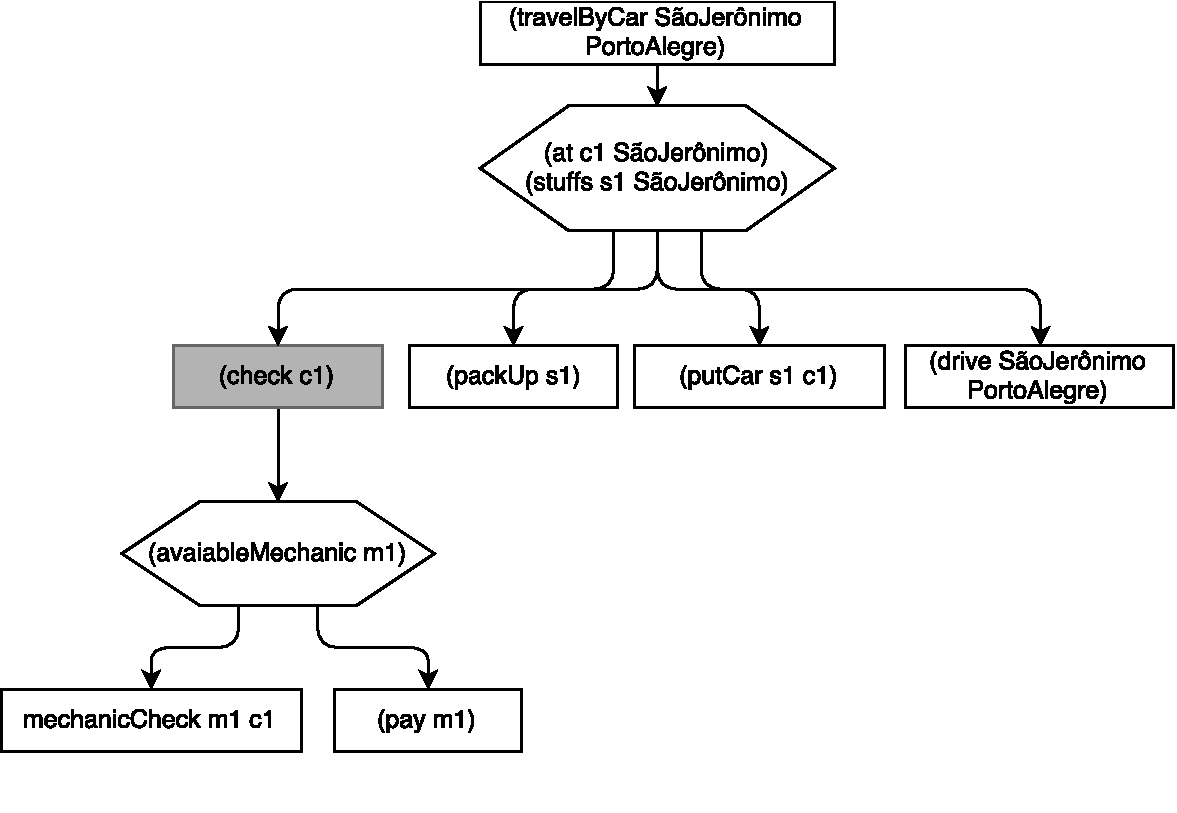
\includegraphics[width=0.7\textwidth]{fig/htnmethodresult.pdf}
	\caption{Arvore de resolução HTN.}
	\label{fig:htnmethodtree}
\end{figure}

O algoritmo de \textit{Total-order Forward Decomposition} (TFD) é utilizado para gerar um plano a partir de uma rede de tarefas inicial com ordenação total, como detalhado no Algoritmo~\ref{alg:tfd}.
O algoritmo gera as ações na mesma ordem que serão executadas, então a cada vez que uma tarefa é alcançada, tudo que antecede a mesma já foi planejado \cite{ghallab2004automated}.
 
\begin{algorithm}
	\caption{Total-order Forward Decomposition}
	\label{alg:tfd}
	\begin{algorithmic}[1]		
		\Function {TFD}{$s, <t_{1}, ...,t_{k}>, O, M$}
			\If {$k = 0$}
				\State	\Return $<>$
			\EndIf
			\If {$t_{1}$ é primitivo}
				\State $ativo = \{(a, b)~ |$ $a$ é uma instancia de $O$ e é aplicável a $s$ e b é uma substituição que torna $a$ relevante para $b(t_{1})\}$
				\If {$ativo = \emptyset$}
					\State \Return falha
				\EndIf
				\State escolhe algum par $(a, b) \in active$
				\State $\pi = TFD(\gamma(s, a), b(<t_{2}, ..., t_{k}>, O, M)$
				\If {$\pi = falha$}
					\State \Return falha
				\Else 
					\State \Return $a . \pi$
			\EndIf
			
			\ElsIf {$t_{1}$ é não primitiva}
				\State $ativo = \{m |~ m$ é aplicável a $s$ e $m \in M\}$
				\If {$ativo = \emptyset$}
					\State \Return falha
				\EndIf
				\State escolhe algum par $(m, b) \in active$
				\State $w =~ $subtarefas$(m).b(<t_{2}, ..., t_{k}>)$
				\State \Return $TFD(s, w, O, M)$
				\EndIf
		\EndFunction
	\end{algorithmic}
\end{algorithm}

\section{AHTN} 

\textit{Adversarial hierarchical-task network} (AHTN) é um algoritmo desenvolvido para lidar com o problema do grande fator de ramificação dos jogos em tempo real~\cite{ontanon2015adversarial} utilizando conhecimento de domínio no estilo de planejamento HTN. 
Nele são combinados técnicas de HTN com o algoritmo \textit{minimax search}. 
O algoritmo assume jogos totalmente observáveis, baseados em turno e determinísticos. 

O Algoritmo~\ref{alg:ahtn}~\cite{ontanon2015adversarial} é a representação da técnica de AHTN, e assume que existem dois jogadores, \textsc{Max} e \textsc{Min}, como no algoritmo de \textit{minimax search} apresentado no Capitulo~\ref{chap:busca}.
O algoritmo também assume uma busca em uma árvore com uma máxima profundidade $d$. 
O intuito do algoritmo de AHTN é gerar os melhores plano para \textsc{Max} e para \text{Min}, junto com o resultado de uma função de avaliação para quando os planos chegam a um estado terminal. 

\begin{algorithm}
	\caption{Adversarial hierarchical-task network}
	\label{alg:ahtn}
	\begin{algorithmic}[1]		
		\Function {AHTNMax}{$s, N_{+}, N_{-}, t_{+}, t_{-}, d$}
		\If {$terminal(s) \vee d \leq 0$}\label{alg:lin:firstLine}
		\State	\Return $(N_{+}, N_{-}, e(s))$
		\EndIf
		\If {$nextAction(N_{+}, t_{+}) \neq \perp$} \label{alg:ahtn:nexaction}
		\State $t = nextAction(N_{+}, t_{+})$ 
		\State \Return $\Call{AHTNMin}{(\gamma(s,t), N_{+}, N_{-}, t, t_{-}, d-1)}$ \label{alg:ahtn:troca}
		\EndIf
		\State $N_{+}^{*} = \perp, N_{-}^{*} = \perp, v^{*} = -\infty$
		\State $\aleph = decompositions_{+}(s, N_{+}, N_{-}, t_{+}, t_{-})$ \label{alg:decompositions}
		\ForAll{$N \in \aleph$} \label{alg:ahtn:for}
		\State $(N^{'}_{+}, N^{'}_{-}, v^{'}) = AHTNMax(s, N, N_{-}, t_{+}, t_{-}, d)$
		\If{$v^{'} > v^{*}$}
		\State $N_{+}^{*} = N^{'}_{+}, N_{-}^{*} = N^{'}_{-}, v^{*} = v^{'} $
		\EndIf
		\EndFor		
		\State \Return $(N_{+}^{*}, N_{-}^{*}, v^{*} )$
		\EndFunction
	\end{algorithmic}
\end{algorithm}

Cada nodo da árvore das jogadas é definido por uma tupla $(s, N_{+}, N_{-}, t_{+}, t_{-})$, onde $s$ é o estado corrente do ambiente, $N_{+}$ e $N_{-}$ são a representação de planos HTN para os jogadores \textsc{Max} e \textsc{Min}, respectivamente, $t_{+}$ e $t_{-}$ representam ponteiros para qual parte do plano HTN está sendo executada, sendo $t_{+}$ para uma tarefa de $N_{+}$ e $t_{-}$ para uma tarefa de $N_{-}$ ~\cite{ontanon2015adversarial}.

A função $nextAction(N,t)$ faz com que, dado uma representação de plano em HTN $N$ e um ponteiro $t$, seja encontrada a próxima tarefa primitiva que deve ser executada em $N$ após a tarefa $t$. Se $t = \perp$ então é retornado a primeira tarefa primitiva a ser executada em $N$. 
Se existir em $N$ alguma tarefas não primitivas e não existir nenhuma tarefa primitiva em $N$ então $nextAction(N,t) = \perp$ \cite{ontanon2015adversarial}.
Na linha~\ref{alg:ahtn:nexaction} é testado se existe alguma tarefa primitiva no plano atual, se existir ela é aplicada e passa para o próximo nível da árvore alternando para \textsc{Min}, através da função $AHTNMin$. 

Um nodo \textsc{Max} $n = (s, N_{+}, N_{-}, t_{+}, t_{-})$ é consistente se as ações primitivas que já estão em $N_{+}$ e $N_{-}$ conseguem ser executadas dado um estado $s$ e uma transição $\gamma$. A definição de consistência de \textsc{Min} é análoga \cite{ontanon2015adversarial}.

Para um nodo \textsc{Max} $n = (s, N_{+}, N_{-}, t_{+}, t_{-})$, $decompositions_{+}(s, N_{+}, N_{-}, t_{+}, t_{-})$ denota o conjunto das decomposições validas que adicionem apenas um novo método em $N_{+}$ (${decompositions(N_{+}, t, m) | m \in applicable(N_{+}, t)}$).
A definição de $decompositions_{-}$ é análoga \cite{ontanon2015adversarial}.
Na linha~\ref{alg:decompositions} é adicionado a $\aleph$ todas as possibilidades de continuação de planos a partir do ponto atual.

Uma função de avaliação $e$, quando aplicada sobre um estado $s \in S$, retorna a recompensa de \textsc{Max} em $s$ se ele for um estado terminal ou uma aproximação se $s$ for um estado não-terminal \cite{ontanon2015adversarial}. 
Na linha~\ref{alg:ahtn:for} são comparados todos os possíveis planos pela função de avaliação e é retornado o melhor plano encontrado para os dois jogadores, junto com o resultado da função de avaliação. 
Quando um estado terminal ou a profundidade for atingida os planos e a função de avaliação para o estado atual são retornados. É o que representa a Linha~\ref{alg:lin:firstLine}

A grande diferença entre o algoritmo de $AHTN$ e o algoritmo do \textit{minimax search}, é que as chamadas recursivas nem sempre se alternam entre \textsc{Max} e \textsc{Min}. 
O algoritmo troca de nodos \textsc{Max} para \textsc{Min} apenas quando os planos estão totalmente decompostos a ponto de gerar uma ação (Linha \ref{alg:ahtn:troca}) \cite{ontanon2015adversarial}.

Para exemplificar o funcionamento do Algoritmo \ref{alg:ahtn}, é apresentado a Figura \ref{fig:ahtn}, que ilustra uma árvore gerada com profundidade $d = 2$. 
Na raiz da árvore pode ser visto que, para os dois jogadores, apenas uma tarefa não primitiva \textit{win} precisa ser decomposta. 
Há duas decomposições que o jogador \textsc{Max} pode aplicar para seu plano HTN, resultando nos nodos $n_{1}$ e $n_{5}$. 
A decomposição de n1 não resulta em nenhuma ação primitiva, e por isso $n_{1}$ continua um nodo \textsc{Max}. 
Uma vez que o jogador \textsc{Max} decompõe sua HTN para o ponto onde a primeira ação pode ser gerada(nodo $n_{2}$ e $n_{5}$), é o turno de \textsc{Min} decompor suas tarefas não primitivas. Quando \textsc{Min} pode gerar suas ações, a profundidade máxima foi atingida (nodos $n_{3}$ e $n_{4}$). 
A função de avaliação $e$ é aplicada para cada um dos estados do jogo para determina o valor das folhas.

\begin{figure}[ht]
	\centering
	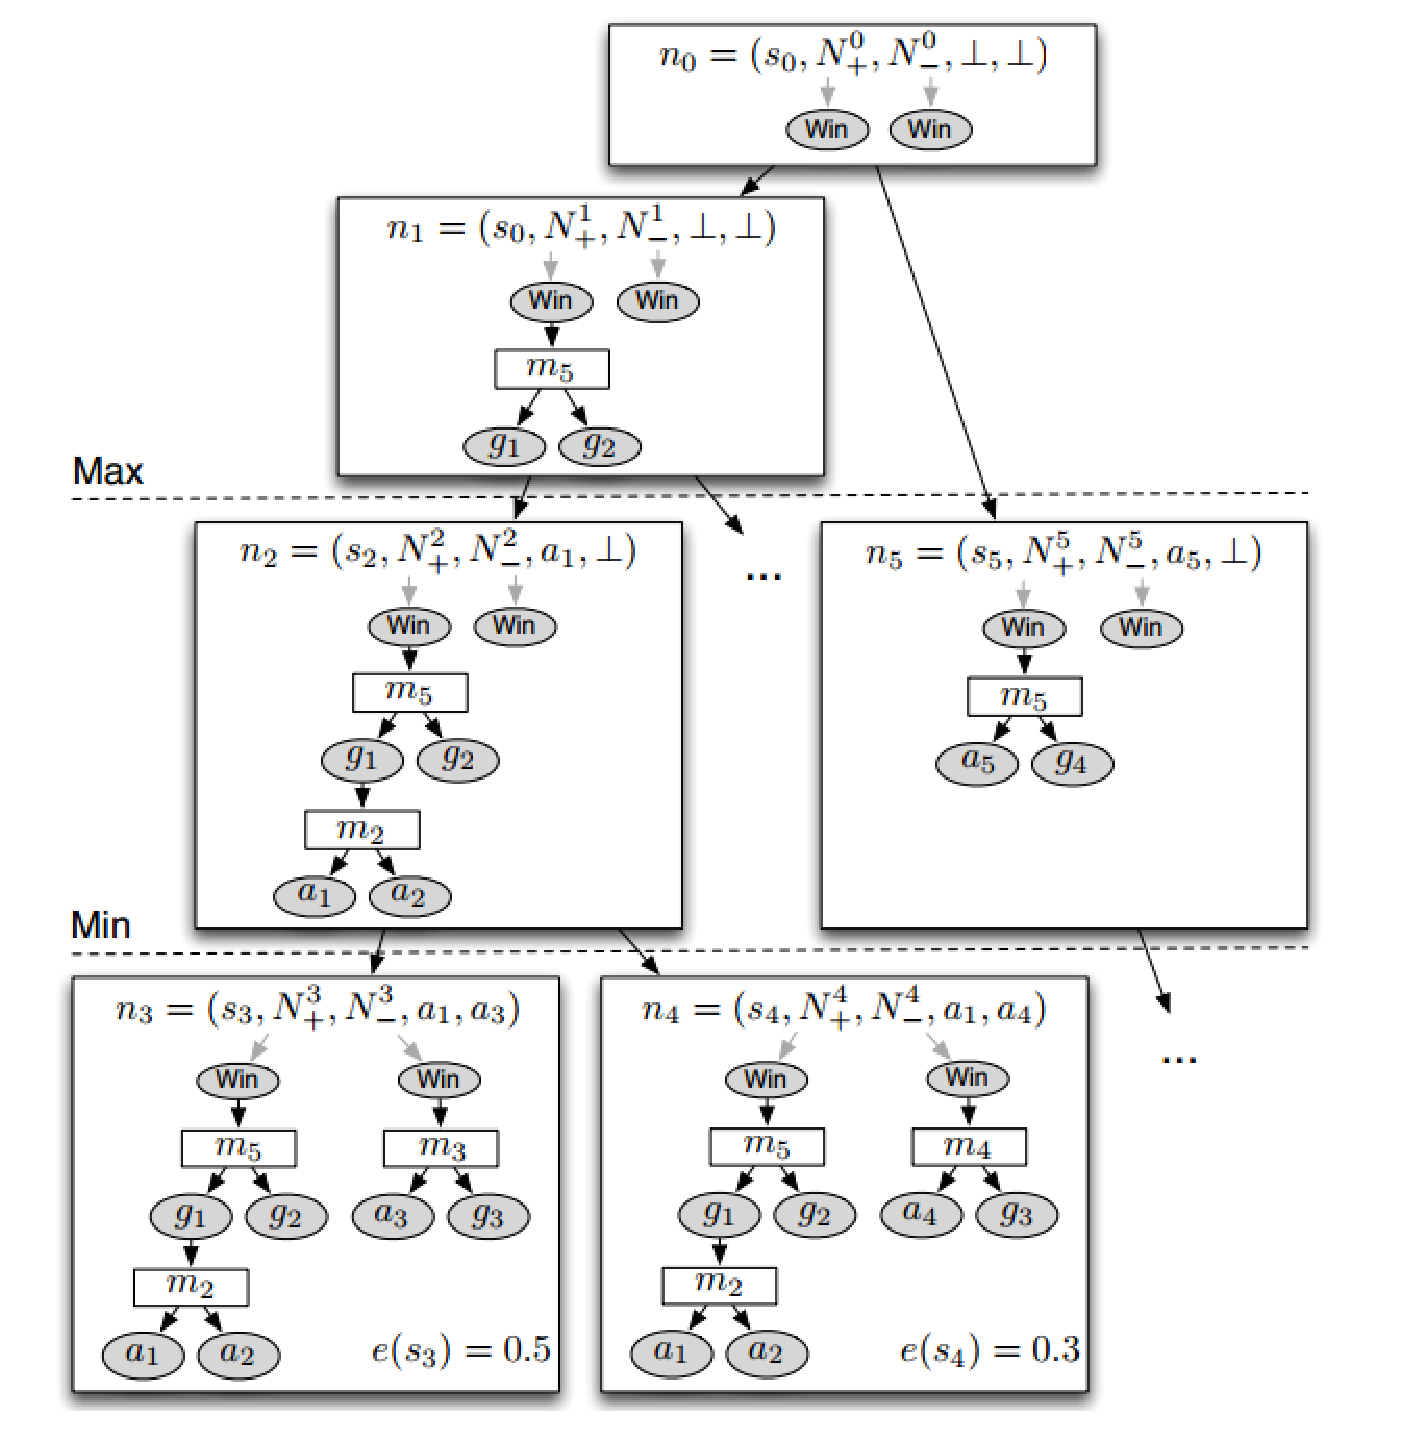
\includegraphics[width=0.6\textwidth]{fig/ahtn.pdf}
	\caption{Árvore gerada pelo algoritmo de AHTN}
	\label{fig:ahtn}
\end{figure}

Em jogos, um agente pode ter que seguir um objetivo, para isso é possível utilizar técnicas de planejamento. O grande problema, continua sendo o grande fator de ramificação e o pouco tempo para determinar a próxima ação do agente \cite{}. O algoritmo de AHTN tenta lidar com esses problemas. 

Com o intuito de aumentar o desempenho do algoritmo, é possível utilizar técnicas de aprendizado de máquina na geração dos planos. No processo de geração do plano é possível ter mais de um método que decomponha a mesma tarefa não primitiva, nesses casos o planejador precisa escolher um dos métodos para tentar chegar ao fim da decomposição. Como dito anteriormente, se em algum ponto, não for possível decompor uma tarefa não primitiva, um retrocesso é feito até chegar a um ponto que outro método possa ser executado. Uma maneira de melhorar a decisão de escolha dos métodos é obtendo uma recompensa a cada decomposição de uma tarefa não primitiva, para que com as informações obtidas nas execuções, as recompensas possam auxiliem nas escolhas dos métodos, com o intuito de minimizar os retrocessos \cite{hogg2010learning}. 